\documentclass[aspectratio=169]{beamer}
\usetheme{Madrid}
\usecolortheme{beaver}
\usepackage[utf8]{inputenc}
\usepackage[T1]{fontenc}
\usepackage{tikz}
\usepackage{amssymb}
\usepackage{graphicx}
\setbeamertemplate{navigation symbols}{}
\setbeamercolor{title}{fg=white,bg=cyan!60!black}
\setbeamercolor{frametitle}{fg=white,bg=cyan!50!black}
\setbeamercolor{block title}{bg=cyan!15,fg=black}
\setbeamercolor{block body}{bg=cyan!5,fg=black}

\title{Story Studio 2 — Style It}
\subtitle{Lesson 1: Paint the Page}
\author{ByteForge --- Grade 7 --- Game Maker}
\date{}

\begin{document}

\begin{frame}
    \titlepage
\end{frame}

\begin{frame}{Content vs. style — two different jobs}
    \Large
    Last week's blocks decided WHAT is on the page. This week's Style blocks decide how it LOOKS — colours, alignment, size.

    \begin{center}
    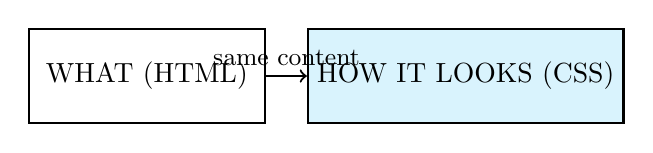
\begin{tikzpicture}[scale=0.9]

        \node[draw, thick, minimum width=3cm, minimum height=1.2cm] (a) at (0,0) {WHAT (HTML)};
        \node[draw, thick, fill=cyan!15, minimum width=3cm, minimum height=1.2cm] (b) at (4.5,0) {HOW IT LOOKS (CSS)};
        \draw[->, thick] (a) -- (b) node[midway, above] {\small same content};
    \end{tikzpicture}
    \end{center}
\end{frame}

\begin{frame}{Content vs. style — two different jobs --- Worked Example}
    \Large
    Worked example: the exact same "My Story" heading, styled two ways — plain black text, or bold cyan text — is still 100\% the same HTML content. Only the CSS rule changed.
\end{frame}

\begin{frame}{Your Turn}
    \Large
    Open the student map, find \textbf{Story Studio 2 — Style It}, and complete
    the \textbf{Paint the Page} challenge --- everything you just saw, they now do themselves.
\end{frame}

\end{document}
